\chapter{Passive Filter Design}
\label{chapter:PassiveFilterDesign}

\section{Introduction}
A filter has to be effectively designed and built to block the unwanted frequencies to a specific speaker cone. This can prevent noise and damage to the cone. Therefore, it is vital to properly design the filters, which begs the question: 'In what manner can filters be effectively created to create the flattest acoustic response?'. A flat acoustic response means that the filters can reproduce the sound at all frequencies with the least change in volume. This would, therefore, help achieve the project's aim, which is to reproduce a sound with the highest accuracy possible. A flat acoustic response can help achieve this, as it will reproduce the sound with the least change in volume possible. Therefore, the filters must be designed to a high standard. This can be done by choosing the most optimal cut-off frequencies, evaluating the best order of the filter, deciding on a Zobel network or not, and selecting the best component values. 
\section{Specifications}
The specifications are that the frequency ranges from 20 to 20 kHz and that the audio is the most accurate possible. This, therefore, leaves the filter groups with a significant amount of flexibility in the design process of the filters. 

\section{Order of filter}
The initial requirement is choosing the order of the filter. This will be the base of the entire filter, as it decides what type of components the filter uses. The order of the filter changes the rate at which its amplitude responds around its cut-off frequencies. The transfer function of a first-order filter will decline by 20 decibels per decade, whereas a second-order filter's transfer function will decline by 40 decibels per decade. 

The significance of the greater decline is that the filter will act closer to an ideal filter, which would therefore make it fit closer to the models made for these filters. This is because, at the cut-off frequency, the filters' amplitude response will decrease to the half-power amplitude quicker with a steeper decline in the amplitude. At and after the half-power amplitude it can be approximated that the frequencies have a negligible impact on the speaker cone, as their power is not enough to make a significant contribution to amplify the sound. Therefore, it was reasoned that a second-order filter was in the best interest of the amplifier, as it would allow the filters to be bound more to the frequencies assigned to them, and have an insignificant impact outside this range. 

\section{Reasoning of Zobel network}
As seen in \ref{fig:/model vs measured impedance}, the impedance of the speaker increases at higher frequencies, which may therefore also cause a voltage increase over the loudspeaker. As a result, it can be said that the sound pressure in the speaker increases cite{IP-manual}. 

To prevent this from affecting the filters, there are two options. The first is taking into account the effect of the frequency-dependent impedance of the speaker. The other option is to connect a Zobel network in parallel with the filter. 

A Zobel network is a connection of elements in parallel with the speaker element so that the combined impedance is fully real. Consequently, the impedance of the speaker will be constant, and simplify calculations.

On the other hand, however, creating a Zobel network is a challenging task, as it requires simulating the network to find the optimal components. Once this is done there are the limitations of the components in the lab, making it unlikely that the Zobel network can fully remove the reactance of the loudspeaker. It may only decrease the frequency dependence of the impedance. Therefore, it was decided by the group that a Zobel network was not appropriate and therefore would not be used.  

\section{Calculation of cut-off frequencies}
Cut-off frequencies are where the transfer function has a gain of $\frac{\sqrt{2}}{2}$, which is considered the -3 dB frequency. For low-pass filters, after this point, frequencies will have a negligible effect on the output. Similarly, for high-pass filters, frequencies before the cut-off frequency have an insignificant impact. Moreover, for the band-pass filter, there are two cut-off frequencies, before the first and after the second, the frequencies are insignificant to the output. 

Deciding on the right cut-off frequencies is of high importance, as the aim of the project is to have the flattest acoustic response. Choosing the right cut-off frequencies plays a significant role in this, as it allows the frequency ranges for each of the speakers to be optimally chosen. Each speaker cone works optimally within a certain frequency range, where tweeters work in high frequencies, bass in low frequencies and mid-toners in between. Frequencies outside the optimal range can create low-quality sound or damage the cone. Therefore, it is important to choose the optimal cut-off frequencies. 

The best cut-off frequencies were chosen by overlaying the acoustic responses of each of the speakers in Python, as seen in \ref{fig: Cutoff frequencies}. Then by observation, and knowledge of the optimal frequency ranges of each of the cones, the cut-off frequencies were decided. This was done by finding where each of the speakers started to become unstable, and finding where the next speaker was stable enough to take over. With constructive and deconstructive interference between the sound waves, it would ultimately result in the flattest response possible.

The decided cut-off frequency for the low pass filter, as seen in fig\ref{fig: Cutoff frequencies} was 200 Hz. This was what we found would give us the flattest overall response. The cut-off frequency for the high-pass filter was 1250 Hz as it would give us a flat transition between the high-pass and band-pass filter. On the other hand, however, it can be noted that at 900 Hz in fig\ref{fig: Cutoff frequencies} there is a large dip in the power response of the mid-toner response. This dip has a significant impact on the overall response before the cut-off frequency. While we attempted to choose the most optimal cut-off frequencies, this dip is something we had to be cautious of. 
\begin{figure}[H]
    \centering
    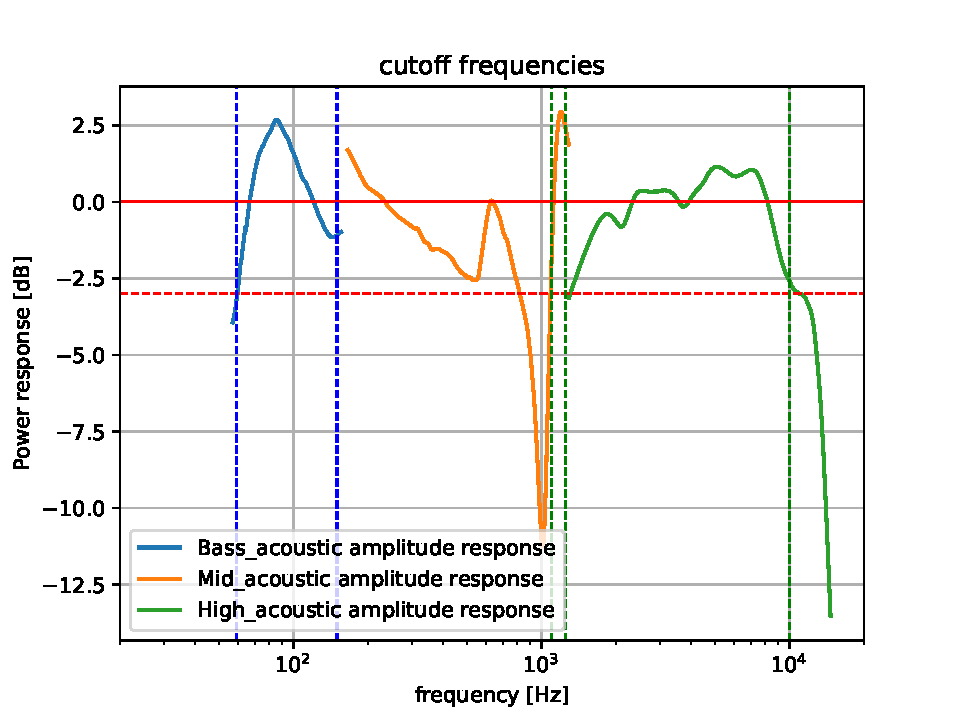
\includegraphics[width=0.6\linewidth]{TU Delft Booming Bass Project Report/figures/FilterGroup/chosenvalues.pdf}
    \captionsetup{justification=raggedright, labelfont=bf}
    \caption{Various amplitude responses plotted to assist in deciding initial cutt-off frequencies}
    \label{fig: Cutoff frequencies}
\end{figure}

\section{Transfer function}
Second-order passive filters are commonly described by their transfer functions, which express the relationship between the output voltage  out and the input voltage. This gives the following equation : 

According to the Kirchoff law 
V_in = V_R +V_L+V_C+V_out
\newline
Where here
\newline 
V_R (t) = R*I(t)  
\newline
V_L (t) = L* dI(t)/dt
\newline 
V_C = 1/c * integral (I(t))
\newline 
v_out = Zspk * I(t)
.




\section{Calculating component values}

\section{Simulations}

\section{Simulation results} %Dit is bode plots en de simulations 

 

\section{Discussion}

\section{Conclusions}

\subsection{Filter Requirements}
 Research question, specifications, reasoning of the required order, calculation
of the cutoff frequencies, reasoning if Zobel network required, transfer function, calculation of
required component values, simulations with nodal analysis, Bode diagrams including phase, discussion incl. comparison between theory, simulations and measurements, and conclusions.




